\section{Introduction}
\label{sec:intro}

Tools such as Claude Code, Codex and OpenCode give a language model an environment in which it can work as an engineer's daily assistant, taking requests and completing them as they come. These agents struggle as requirements accumulate. On EvoCode-Bench, pass rates fall below half of round-1 performance by round 5~\cite{shen2026evocode}. On SlopCodeBench, structural erosion rises in 77\% of trajectories~\cite{orlanski2026slopcode}. The problem appears to sit in the code as well as the conversation: ChainSWE finds that inherited repository state accounts for most of the decline~\cite{jin2026chainswe}, and SlopCodeBench reports that quality prompts lower the starting point of degradation but not its rate. Both suggest that revisiting the design is a research direction worth exploring.

Any engineer knows the feeling behind those numbers. By the tenth request you can see how you would have designed your system if you had known all of the requirements, but you are too far in, and you have a next request to get to. You could copy all of your requirements into a new session and start over, but that throws away everything the agent has learned about your project. Hindsight presents a solution to combat these problems. The system is designed so that you talk to the main agent in your session as normal, and in the background a team of agents does the starting over, then hands what it found back to the main agent, which knows the latest code and can decide, along with the user, what is worth keeping (Figure~\ref{fig:timeline}).

\begin{figure}[t]
  \centering
  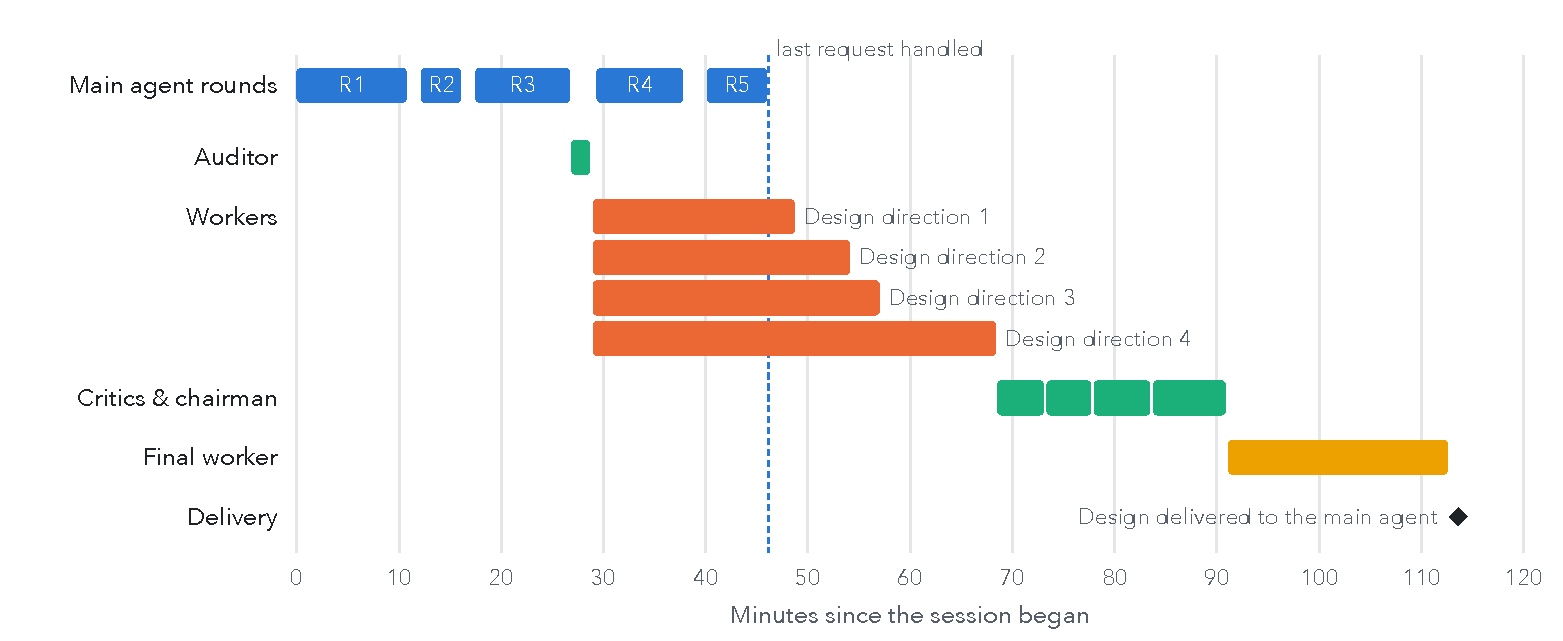
\includegraphics[width=0.88\linewidth]{fig_timeline.pdf}
  \caption{How a background run overlaps with a session. The user keeps working while the workers, the review and the final worker run, so a design can arrive well after the request that prompted it.}
  \label{fig:timeline}
\end{figure}

This doesn't happen on every request. That would create too much noise and disrupt the user's attention, and most requests are direct enough for the main agent to handle, or are simply questions for it. The intelligence of the system lies in figuring out when it makes sense to try something new, and in only sending something back when the redesign is useful.

The design also relies on cheap tokens. The background agents run open-source models in Sailboxes that bill only for what they use, so the user doesn't have to worry about a background system blowing up their costs. A system like this is enabled by cheap intelligence, and it becomes more useful as intelligence gets cheaper.
